
%%% main document {{{

\documentclass[
a4paper,     %% defines the paper size: a4paper (default), a5paper, letterpaper, ...
% landscape,   %% sets the orientation to landscape
% twoside,     %% changes to a two-page-layout (alternatively: oneside)
% twocolumn,   %% changes to a two-column-layout
 headsepline, %% add a horizontal line below the column title
% footsepline, %% add a horizontal line above the page footer
% titlepage,   %% only the titlepage (using titlepage-environment) appears on the first page (alternatively: notitlepage)
% parskip,     %% insert an empty line between two paragraphs (alternatively: halfparskip, ...)
% leqno,       %% equation numbers left (instead of right)
% fleqn,       %% equation left-justified (instead of centered)
% tablecaptionabove, %% captions of tables are above the tables (alternatively: tablecaptionbelow)
% draft,       %% produce only a draft version (mark lines that need manual edition and don't show graphics)
% 10pt         %% set default font size to 10 point
11pt         %% set default font size to 11 point
% 12pt         %% set default font size to 12 point
]{scrartcl}  %% article, see KOMA documentation (scrguide.dvi)



%%%%%%%%%%%%%%%%%%%%%%%%%%%%%%%%%%%%%%%%%%%%%%%%%%%%%%%%%%%%%%%%%%%%%%%%%%%%%%%%
%%%
%%% packages
%%%

%%%
%%% encoding and language set
%%%

%%% ngerman: language set to new-german
\usepackage{ngerman}

%%% babel: language set (can cause some conflicts with package ngerman)
%%%        use it only for multi-language documents or non-german ones
%\usepackage[ngerman]{babel}

%%% inputenc: coding of german special characters
\usepackage[utf8]{inputenc}

%%% fontenc, ae, aecompl: coding of characters in PDF documents
\usepackage[T1]{fontenc}
\usepackage{ae,aecompl}

%%%
%%% technical packages
%%%

%%% amsmath, amssymb, amstext: support for mathematics
%\usepackage{amsmath,amssymb,amstext}

%%% psfrag: replace PostScript fonts
\usepackage{psfrag}

%%% listings: include programming code
\usepackage{listings}
\usepackage{courier}
\lstset{basicstyle=\footnotesize\ttfamily,breaklines=true}

%%% units: technical units
\usepackage{units}

%%% tiefgestellte zahlen
\usepackage{subscript}

%%% mathefoo
\usepackage{amsmath}

%%% landscape page
\usepackage{pdflscape}

%%% multirow table stuff
\usepackage{multirow}
\usepackage{array}

\usepackage{xcolor}
% TikZ-Bibliotheken
\usepackage{tikz}
 \usetikzlibrary{backgrounds}
 \usetikzlibrary{matrix}
 \usetikzlibrary{circuits.ee.IEC}
 \usetikzlibrary{circuits.logic.IEC}
 \usetikzlibrary{positioning}
 
 
%Hintergrundstyle - optional
\tikzstyle{background rectangle}=
  [thick,draw=\lightgray, fill=white!99!black, rounded corners]
 
%Volt- und Amperemeter festlegen:
\tikzset{circuit declare symbol = ammeter}
\tikzset{set ammeter graphic ={draw,generic circle IEC, minimum size=5mm,info=center:A}}
\tikzset{circuit declare symbol = voltmeter}
\tikzset{set voltmeter graphic ={draw,generic circle IEC, minimum size=5mm,info=center:V}}
\tikzset{circuit declare symbol = generator}
\tikzset{set generator graphic ={draw,rectangle ee, minimum size=5mm,info=center:G}}

%%%%%%%%%%%%%%%%%%%%%%%%%%%%%%%%%%%%%%%%%%%%%%%%%%%%%%%%%%%%%%%%%%%%%%%%%%
% Transistor Platzhalter, bitte durch echten Transistor ersetzen
\tikzset{circuit declare symbol = transistor}
\tikzset{set transistor graphic ={draw,generic circle IEC, minimum size=5mm,info=center:T}}
%%%%%%%%%%%%%%%%%%%%%%%%%%%%%%%%%%%%%%%%%%%%%%%%%%%%%%%%%%%%%%%%%%%%%%%%


% Spannungs und Strompfeile
\tikzset{
  Pfeil/.style={thick,shorten >=#1,shorten <=#1,->}, % für Peile
  UPfeil/.style={blue,Pfeil=#1,font={\sffamily\itshape}},% für Spannungspfeile
  IPfeil/.style={red,Pfeil=#1,font={\ttfamily\itshape}} % für Strompfeile
}


%\usepackage{circuitikz}

%Boxen
\usepackage{empheq}
 
% Command "alignedbox{}{}" for a box within an align environment
% Source: http://www.latex-community.org/forum/viewtopic.php?f=46&t=8144
\newlength\dlf  % Define a new measure, dlf
\newcommand\alignedbox[2]{
% Argument #1 = before & if there were no box (lhs)
% Argument #2 = after & if there were no box (rhs)
&  % Alignment sign of the line
{
\settowidth\dlf{$\displaystyle #1$}  
    % The width of \dlf is the width of the lhs, with a displaystyle font
\addtolength\dlf{\fboxsep+\fboxrule}  
    % Add to it the distance to the box, and the width of the line of the box
\hspace{-\dlf}  
    % Move everything dlf units to the left, so that & #1 #2 is aligned under #1 & #2
\boxed{#1 #2}
    % Put a box around lhs and rhs
}
}

%%%
%%% layout
%%%

%%% scrpage2: KOMA heading and footer
%%% Note: if you don't use this package, please remove 
%%%       \pagestyle{scrheadings} and corresponding settings
%%%       below too.
\usepackage[automark]{scrpage2}


%%%
%%% PDF
%%%

\usepackage{ifpdf}

%%% Should be LAST usepackage-call!
%%% For docu on that, see reference on package ``hyperref''
\ifpdf%   (definitions for using pdflatex instead of latex)

  %%% graphicx: support for graphics
  %\usepackage[pdftex]{graphicx}

  \pdfcompresslevel=9

  %%% hyperref (hyperlinks in PDF): for more options or more detailed
  %%%          explanations, see the documentation of the hyperref-package
  \usepackage[%
    %%% general options
    pdftex=true,      %% sets up hyperref for use with the pdftex program
    %plainpages=false, %% set it to false, if pdflatex complains: ``destination with same identifier already exists''
    %
    %%% extension options
    backref,      %% adds a backlink text to the end of each item in the bibliography
    pagebackref=false, %% if true, creates backward references as a list of page numbers in the bibliography
    colorlinks=true,   %% turn on colored links (true is better for on-screen reading, false is better for printout versions)
    %
    %%% PDF-specific display options
    bookmarks=true,          %% if true, generate PDF bookmarks (requires two passes of pdflatex)
    bookmarksopen=false,     %% if true, show all PDF bookmarks expanded
    bookmarksnumbered=false, %% if true, add the section numbers to the bookmarks
    %pdfstartpage={1},        %% determines, on which page the PDF file is opened
    pdfpagemode=None         %% None, UseOutlines (=show bookmarks), UseThumbs (show thumbnails), FullScreen
  ]{hyperref}


  %%% provide all graphics (also) in this format, so you don't have
  %%% to add the file extensions to the \includegraphics-command
  %%% and/or you don't have to distinguish between generating
  %%% dvi/ps (through latex) and pdf (through pdflatex)
  \DeclareGraphicsExtensions{.pdf}

\else %else   (definitions for using latex instead of pdflatex)

  \usepackage[dvips]{graphicx}

  \DeclareGraphicsExtensions{.eps}

  \usepackage[%
    dvips,           %% sets up hyperref for use with the dvips driver
    colorlinks=false %% better for printout version; almost every hyperref-extension is eliminated by using dvips
  ]{hyperref}

\fi


%%% sets the PDF-Information options
%%% (see fields in Acrobat Reader: ``File -> Document properties -> Summary'')
%%% Note: this method is better than as options of the hyperref-package (options are expanded correctly)
\hypersetup{
  pdftitle={}, %%
  pdfauthor={}, %%
  pdfsubject={}, %%
  pdfcreator={Accomplished with LaTeX2e and pdfLaTeX with hyperref-package.}, %% 
  pdfproducer={}, %%
  pdfkeywords={} %%
}


%%%%%%%%%%%%%%%%%%%%%%%%%%%%%%%%%%%%%%%%%%%%%%%%%%%%%%%%%%%%%%%%%%%%%%%%%%%%%%%%
%%%
%%% user defined commands
%%%

%%% \mygraphics{}{}{}
%% usage:   \mygraphics{width}{filename_without_extension}{caption}
%% example: \mygraphics{0.7\textwidth}{rolling_grandma}{This is my grandmother on inlinescates}
%% requires: package graphicx
%% provides: including centered pictures/graphics with a boldfaced caption below
%% 
\newcommand{\mygraphics}[3]{
  \begin{center}
    \includegraphics[width=#1, keepaspectratio=true]{#2} \\
    \textbf{#3}
  \end{center}
}

%%%%%%%%%%%%%%%%%%%%%%%%%%%%%%%%%%%%%%%%%%%%%%%%%%%%%%%%%%%%%%%%%%%%%%%%%%%%%%%%
%%%
%%% define the titlepage
%%%

% \subject{}   %% subject which appears above titlehead
% \titlehead{} %% special heading for the titlepage

%%% title
\title{BFK-L CAT Projekt}

%%% author(s)
\author{Felix Schiller \\ Tilman Frey \\ E2FS2}

%%% date
\date{Reutlingen, am 17.10.2016}

% \publishers{}

% \thanks{} %% use it instead of footnotes (only on titlepage)

% \dedication{} %% generates a dedication-page after titlepage


%%% uncomment following lines, if you want to:
%%% reuse the maketitle-entries for hyperref-setup
%\newcommand\org@maketitle{}
%\let\org@maketitle\maketitle
%\def\maketitle{%
%  \hypersetup{
%    pdftitle={\@title},
%    pdfauthor={\@author}
%    pdfsubject={\@subject}
%  }%
%  \org@maketitle
%}


%%%%%%%%%%%%%%%%%%%%%%%%%%%%%%%%%%%%%%%%%%%%%%%%%%%%%%%%%%%%%%%%%%%%%%%%%%%%%%%%
%%%
%%% set heading and footer
%%%

%%% scrheadings default: 
%%%      footer - middle: page number
\pagestyle{scrheadings}

%%% user specific
%%% usage:
%%% \position[heading/footer for the titlepage]{heading/footer for the rest of the document}

%%% heading - left
\ihead[]{Schiller, Felix \\ Frey, Tilman}

%%% heading - center
\chead[]{BFK-L \\ CAT-Projekt}

%%% heading - right
\ohead[]{\thepage}

%%% footer - left
% \ifoot[]{}

%%% footer - center
% \cfoot[]{}

%%% footer - right
% \ofoot[]{}



%%%%%%%%%%%%%%%%%%%%%%%%%%%%%%%%%%%%%%%%%%%%%%%%%%%%%%%%%%%%%%%%%%%%%%%%%%%%%%%%
%%%
%%% begin document
%%%

\begin{document}

% \pagenumbering{roman} %% small roman page numbers

%%% include the title
% \thispagestyle{empty}  %% no header/footer (only) on this page
\maketitle

%%% start a new page and display the table of contents
\newpage
\tableofcontents

%%% start a new page and display the list of figures
% \newpage
% \listoffigures

%%% start a new page and display the list of tables
% \newpage
% \listoftables

%%% display the main document on a new page 
\newpage

% \pagenumbering{arabic} %% normal page numbers (include it, if roman was used above)

%%%%%%%%%%%%%%%%%%%%%%%%%%%%%%%%%%%%%%%%%%%%%%%%%%%%%%%%%%%%%%%%%%%%%%%%%%%%%%%%
%%%
%%% begin main document
%%% structure: \section \subsection \subsubsection \paragraph \subparagraph
%%%
\section{Kundenauftrag}
Im Foyer eines IT-Dienstleisters soll ein Hausnetzwerk (CAT5) mit einem Patchfeld und zwei Datendosen (UAE 8/8) ausgestellt werden.  
Es wird ein Ausstellungsstück mit Patchpanel, Brüstungskanal und zwei Doppeldatendosen hergestellt. 
Die Planung und Dokumentation wird in diesem Dokument abgelegt.
Als Demonstration wird mithilfe der Verkabelung ein P2P-Netzwerk mit Laufwerksfreigabe eingerichtet.


\section{Materialien und Werkzeuge}
\subsection{Werkzeuge}
Um die arbeiten an Leitungen, Anschlussdosen und Patchfeldern möglichst effizient zu gestalten empfiehlt es sich die passenden, teilweise spezialisierten Werkzeuge zu verwenden.
\begin{itemize}
	* Seitenschneider klein und groß \\
	* Schraubendreher Plus-Minus \\
	* Schlitzschraubendreher \\
	* Abisolierer \\
	* Anlegewerkzeug LSA-Plus \\
	* TDR Messgerät
\end{itemize}
Schraubendreher, Seitenschneider und Abisolierzange sollten allgemein bekannt sein. 
Das Anlegewerkzeug LSA-Plus und das TDR Messgerät sind spezialisierte Werkzeuge die hauptsächlich in der Netzwerktechnik eingesetzt werden.

\subsubsection{Anlegewerkzeug LSA-Plus}
Die Abkürzung LSA steht für Löt-, Schraub- und Abisolierfrei und bezeichnet eine im Jahr 1980 zum Patent angemeldetes Verfahren zum Kontaktieren von Leitungen in der Fernmeldetechnik.
Wie später noch bei der Dose und beim Patchfeld genauer beschrieben können nach diesem Verfahren die einzelnen Adern des Verlegekabels schnell und einfach verbunden, auch aufgelegt oder Angelegt werden.

\begin{figure}[htbp] 
	\centering
	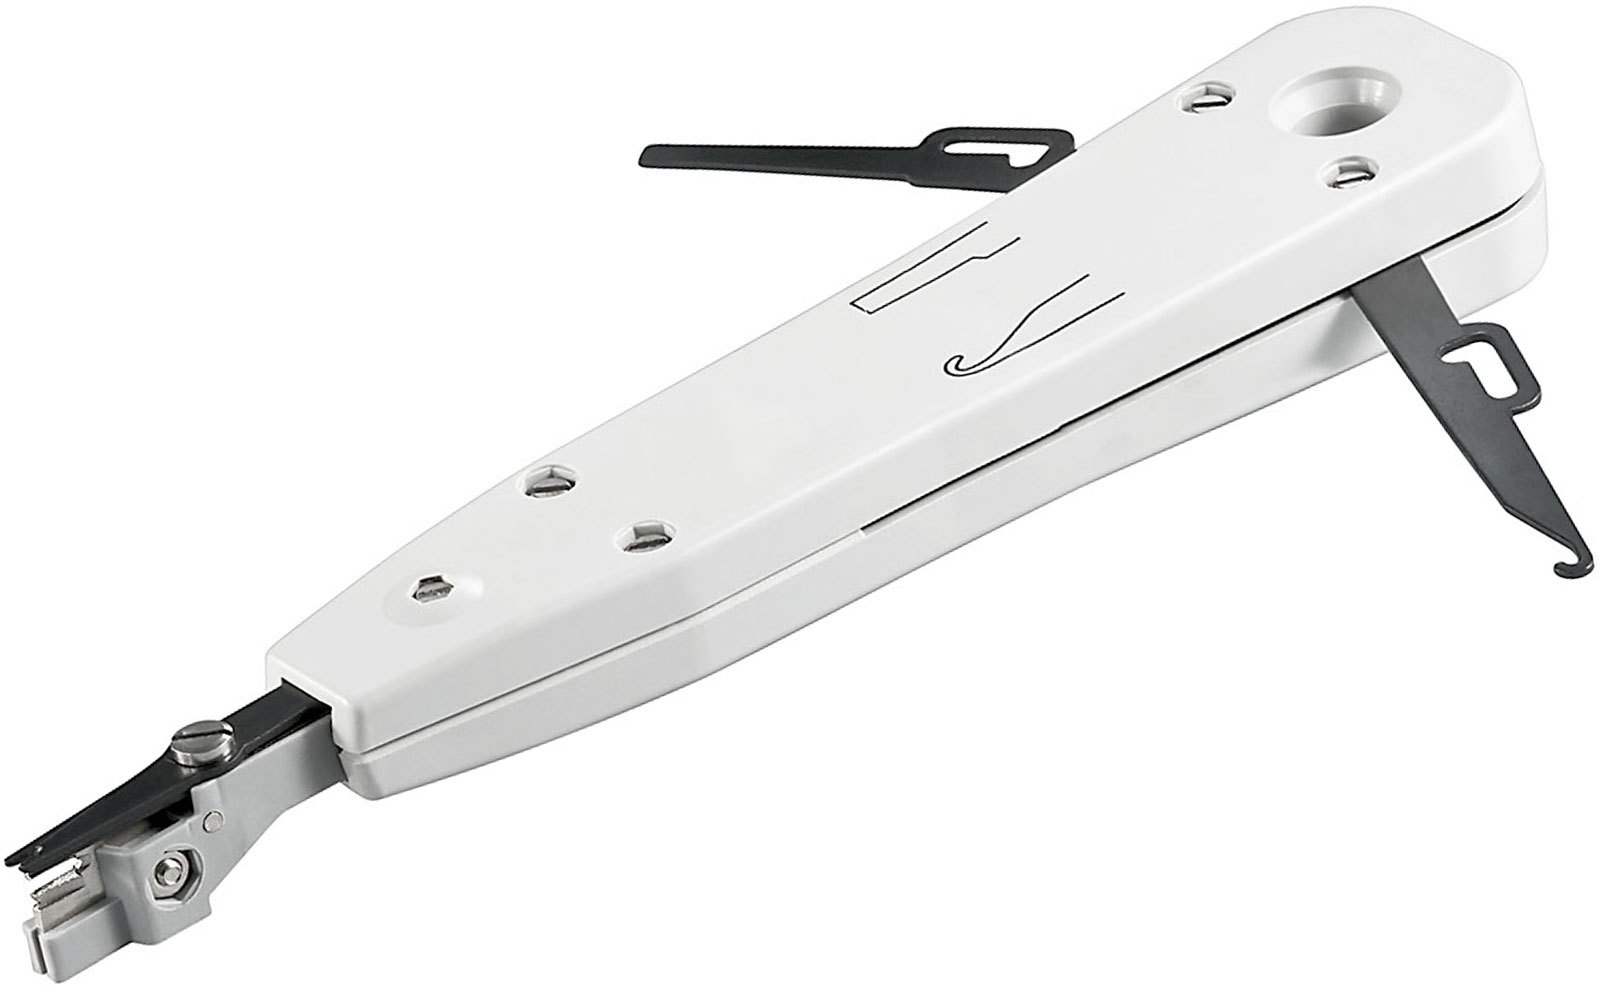
\includegraphics[width=0.7\textwidth]{lsa-werkzeug.jpeg}
	\caption{LSA-Werkzeug von Krone}
	\label{fig:LSA1}
\end{figure}

Das Ganze geschieht mithilfe des Anlegewerkzeugs, das mehrere Funktionen in sich vereint.
Die Spitze, im Bild links unten, dient dazu die Ader zwischen die Schneidklemmen einzuführen.
Mit dem etwas breiteren Kunststoffblock unten wird die Ader zentriert, das schlankere Teil darüber ist schmal genug um zwischen die schneidkemmen zu gleiten.
Sobald durch den Anwender genügend Kraft aufgewendet und die Ader ganz zwischen die Schneidklemmen gedrückt wurde, löst die Schere, im Bild oben auf, aus und kürzt die Ader auf die passende Länge.
Sollte eine Ader in der falschen Klemme gelandet sein, kann sie mithilfe des Hakens, im Bild rechts, wieder aus der Klemme gezogen werden. 


\subsubsection{TDR-Messgerät}
Ein Time-Domain-Reflectometer, abgekürzt TDR ist ein Messgerät, das Reflexionscharakteristika von elektromagnetischen Wellen und Signalen in Kabeln misst. 
Diese Messgeräte finden als Abnahmekontrolle in neuverkabelten Gebäuden eine große Rolle.

Das Messgerät besteht aus zwei wesentlichen Bauteilen. 
Zum einen das  Handgerät, in dem die Auswerteelektronik, Display und Stromquelle untergebracht sind und zum anderen eine abgesetzte Einheit zum Abschluss des durchzumessenden Kabeles.
Die abgesetzte Einheit simuliert durch ihre elektrischen Eigenschaften die Netzwerkschnittstelle eines Switches oder Rechners.
Das Handgerät sendet eine Folge von sehr kurzen Spannungspulsen in die Einzeladern des zu testenden Kabels.
Die Spannungspulse sind dabei so weit auseinander, dass die Echos aller früheren Impulse abgeklungen sind. 
Aber gerade die Echos der Impulse, die auf der Leitung hin und herwandern sind für die Fehlersuche interessant.
An kurzgeschlossenen Kabelenden zum Beispiel kehrt sich die Polarisierung des Impulses an der Fehlerstelle um. 
Quetschungen oder andere Verletzungen des Kabels können zur Teilreflexion des Impulses führen. 
Die Laufzeit des Impulses bis zur Fehlerstelle oder bis zur abgesetzten Abschlusseinheit gibt Auskunft über die Leitungslänge. 
So lässt sich schnell die Fehlerstelle in dem verlegten Kabel lokalisieren und reparieren.
Neben der Impulsantwort überprüft das Messgerät noch den durchgang aller acht Adern sowie des Schirms und deckt dabei eventuell nicht verbundene Adern oder Kurzschlüsse zur Schirmung auf.

Anhand aller gesammelter Messergebnisse kann der Verbund aus Patchfeld, Leitung und Anschlussdose vom Gerät automatisch in eine der Kategorien CAT 5 bis CAT 7 einsortiert werden.



\subsection{Materialien}
\subsubsection{Patchfeld}
Modell Patchfeld: BTR E-DAT 6x8 CAT6 \\
Das im Ausstellungsstück verwendete Patchfeld ist ein 6 Port-Aufputz Verteiler und Anschlussdose für die strukturierte Gebäudeverkabelung, hergestellt von BTR, verwendet. 
Das Patchfeld ist CAT.6 Klassifiziert und damit für 10GBit Ethernet und HDBaseT geeignet. 
Es zeichnet sich durch besonders einfache Auflegemöglichkeit aus, da die Adernpaare ohne Aufdrehen der Verseilung bis zur LSA-Klemme geführt werden können.

Die LSA Klemme besteht aus einem z-förmig ausgebildeten Anschlusselement aus Metall.
Die geraden Teile des Z, im verwendeten Patchfeld unter weißem Kunststoff versteckt, dienen als Klemmrippen und halten die Schneidklemmen von Aderbewegungen frei.
Der eigentliche Kontaktierungsteil der Klemme steht ca im $45^{\circ}$-Winkel zur Aderachse.
Die scharfen Kanten in der metallenen Schneidklemmen schneiden durch die Isolierung der Ader und es entsteht eine elektrisch leitfähige Verbindung.
Diese Verbindung ist kaltverschweißt und gasdicht, sodass keine Korrosion auftreten kann und eine Dauerhafte Verbindung bestehen bleibt.

Die Klemmen sind mit der Adernfarbe nach TIA/EIA 568A gekennzeichnet und beschriftet, sodass ohne Nachschlagen der Belegung im Datenblatt direkt aufgelegt werden kann.

\begin{figure}[htbp] 
	\centering
	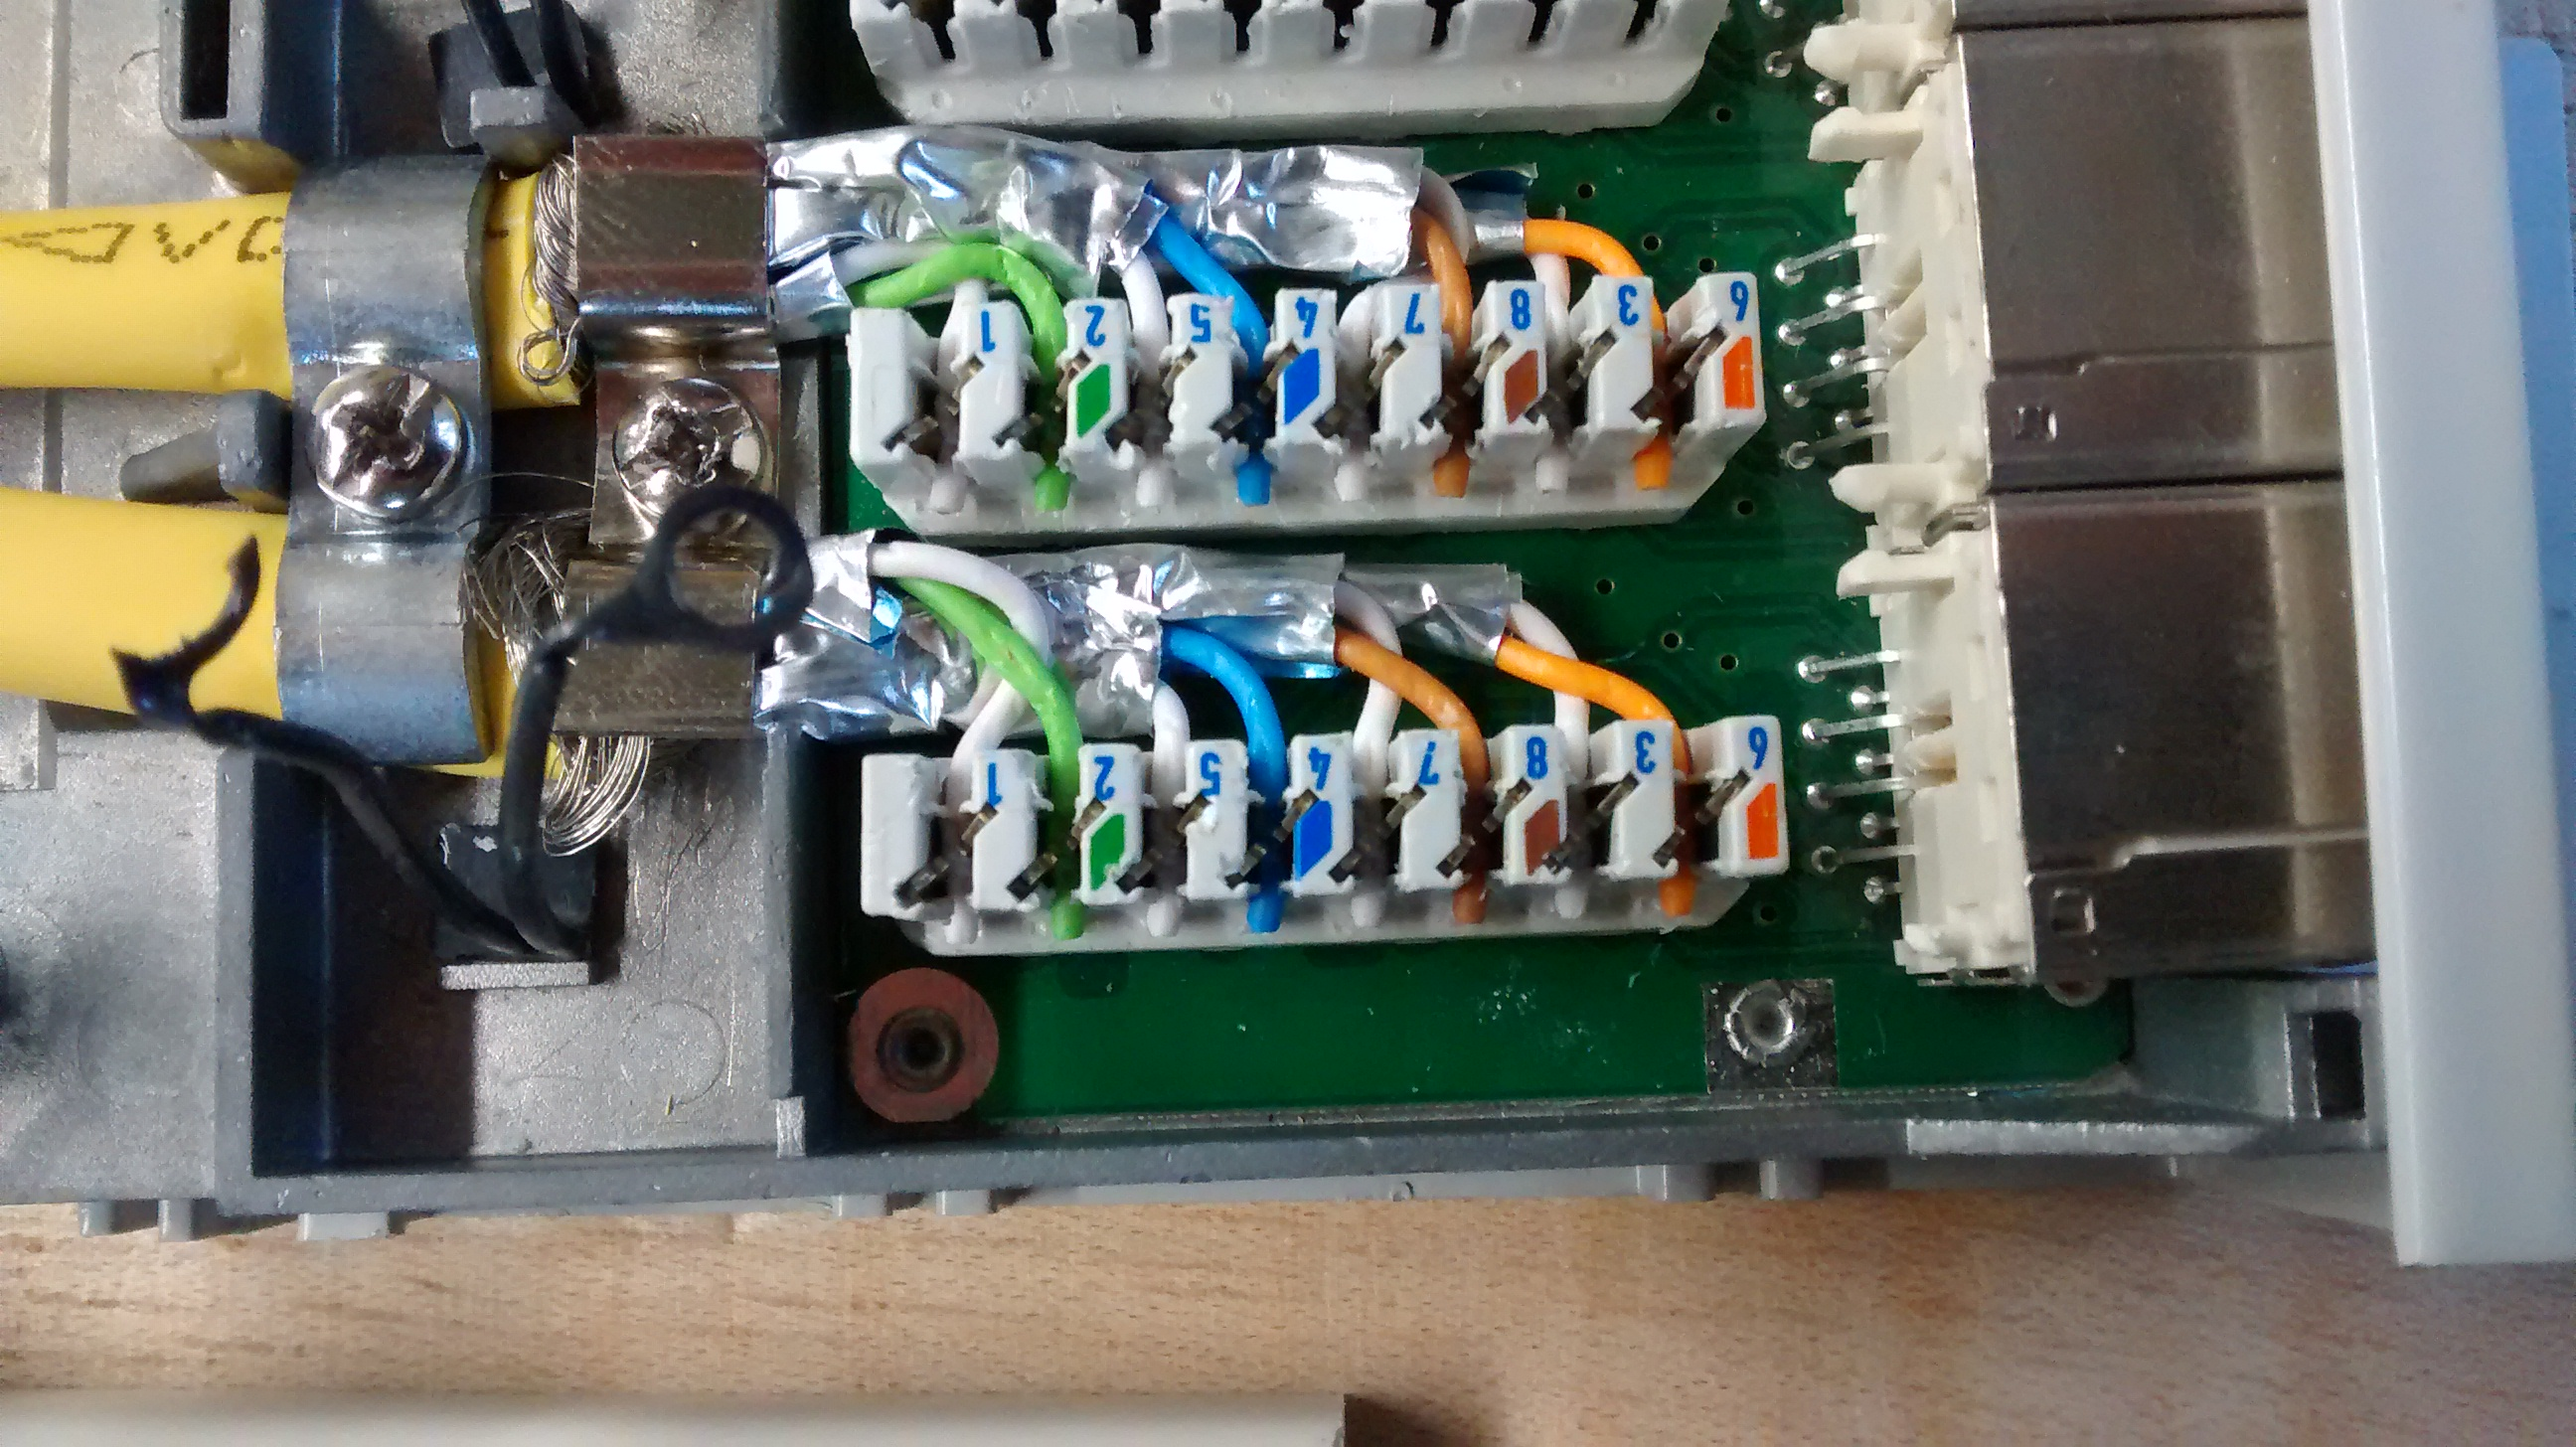
\includegraphics[width=0.7\textwidth]{patchfeld.jpg}
	\caption{Zwei aufgelegte Verlegekabel am Patchfeld}
	\label{fig:Kabel1}
\end{figure}

\subsubsection{Datendose}
TODO: Modell Dose rausfinden \\

\begin{figure}[htbp] 
	\centering
	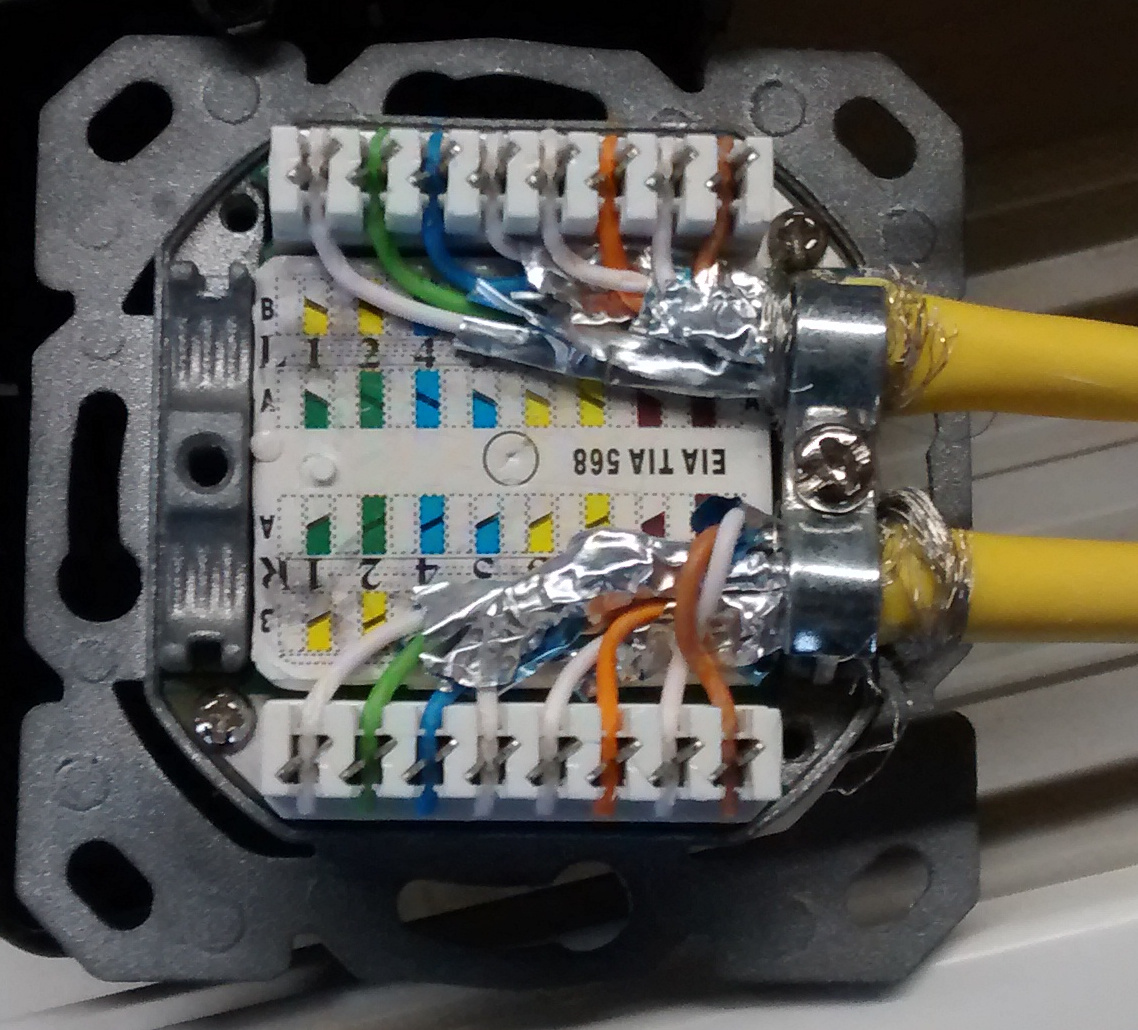
\includegraphics[width=0.7\textwidth]{anschlussdose.jpg}
	\caption{Aufgelegte Datendose}
	\label{fig:Dose1}
\end{figure}

\subsubsection{Verlegekabel}
ELTROPA net-works 1000 Cat.7 1000MHz 4x2xAWG23 HF3

Text tippen
\begin{figure}[htbp] 
	\centering
	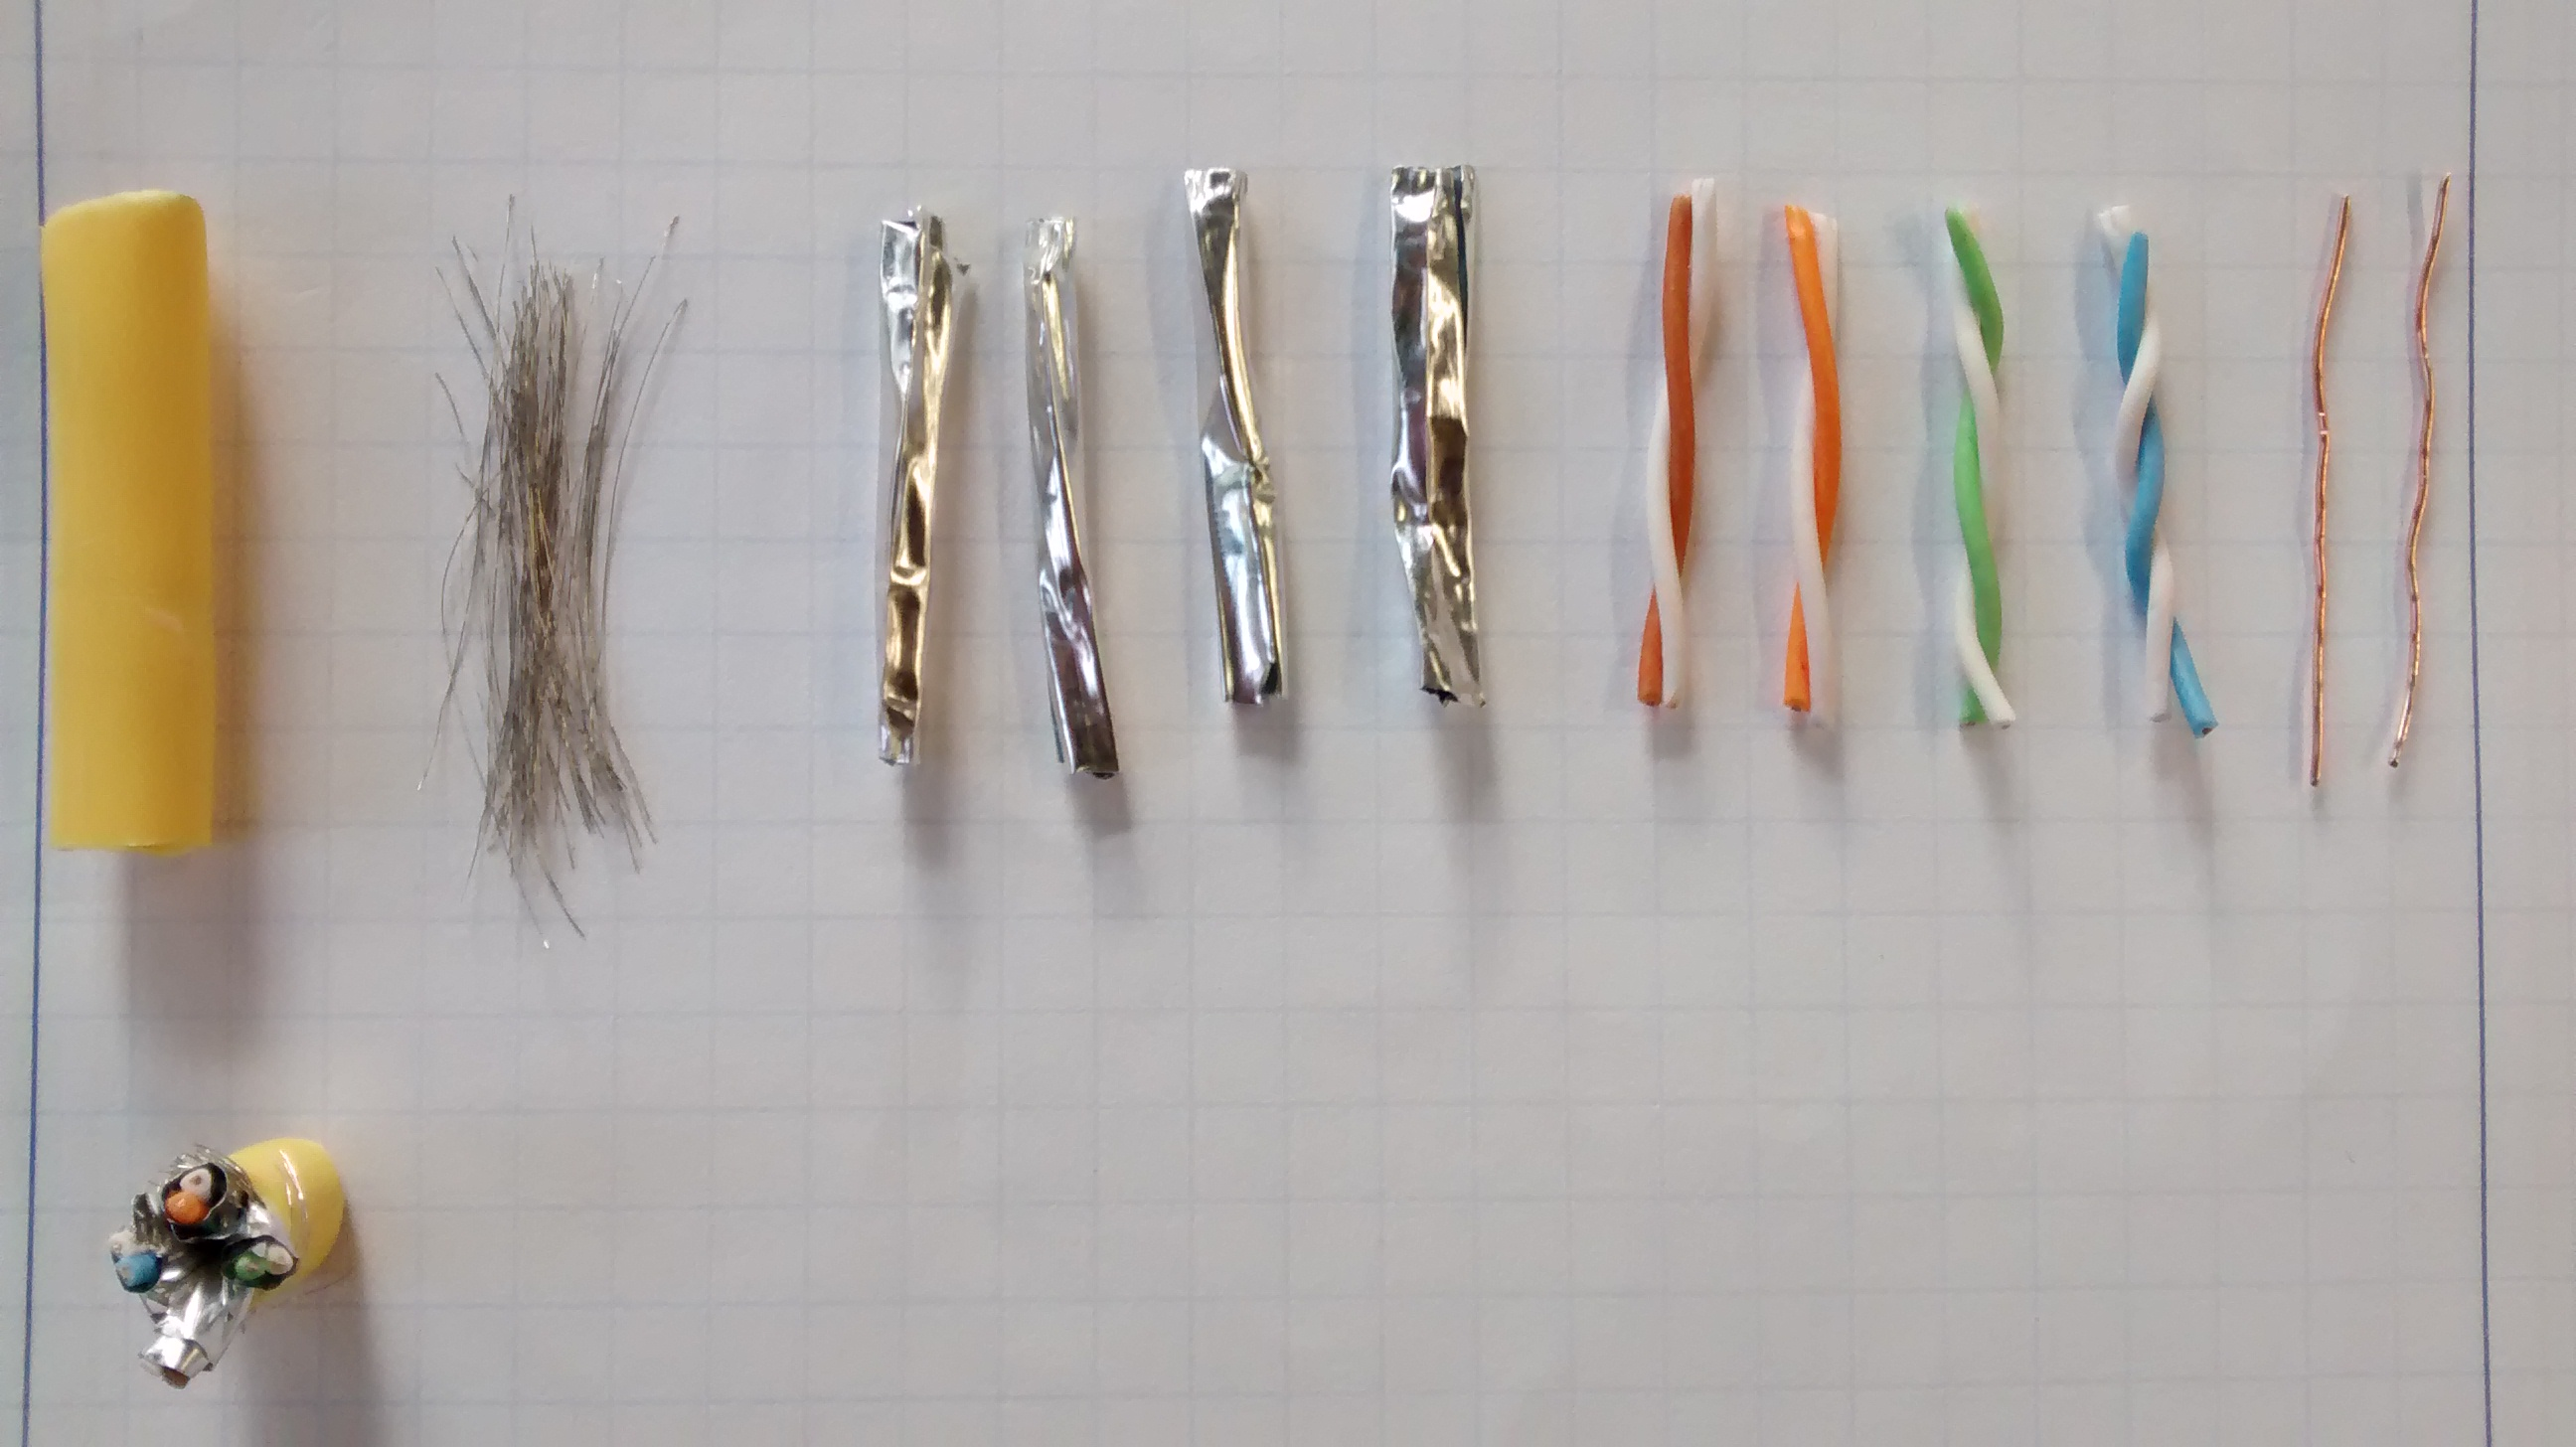
\includegraphics[width=0.7\textwidth]{verlegekabel.jpg}
	\caption{Verlegekabel in einzelne Komponenten zerlegt}
	\label{fig:Kabel1}
\end{figure}


\section{Zeitplanung}
\subsection{Ursprüngliche Planung}
\begin{tabular}{ r | l }
	\hline 
	Zeit &	Aufgabe \\ \hline
	2.0h &	Recherche zu Materialien und Werkzeugen \\
	0.5h &	Aufstellen der Zeitplanung des Projekts \\
	1.0h &	Erstellen des Verdrahtungs- und Aufbauplan \\
	2.5h &	Aufbau der Verkabelung und überprüfung \\
	1.0h &	Einrichten der Dateifreigabe \\
	4.0h &	Dokumentation und Erstellung der Präsentation \\
	0.5h & 	Präsentation \\
	\hline
\end{tabular}


\subsection{Tatsächliche Arbeitszeit TODO}
\begin{tabular}{ r | l }
	\hline 
	Zeit &	Aufgabe \\ \hline
	2.0h &	Recherche zu Materialien und Werkzeugen \\
	0.5h &	Aufstellen der Zeitplanung des Projekts \\
	1.0h &	Erstellen des Verdrahtungs- und Aufbauplan \\
	6.0h &	Aufbau der Verkabelung und Überprüfung \\
	1.5h &	Einrichten der Dateifreigabe \\
	4.0h &	Dokumentation und Erstellung der Präsentation \\
	0.5h & 	Präsentation \\
	\hline
\end{tabular}

\section{Kostenkalkulation}
blub Einkauf, Verkauf, Handelskalkulation …

\section{Aufbau- und Verdrahtungsplan}
Das aufgebaute Ausstellungsstück stellt einen Teil der Tertiärverkabelung dar, wenn man die strukturierte Verkabelung nach der Europäischen Norm EN 50173-1 für Anwendungsneutrale Kommunikationskabelanlagen, oder die nordamerikanische Norm TIA/EIA 568 zugrunde legt.
Die Tertiärverkabelung umfasst die horizontale Verkabelung innerhalb eines Stockwerks und wird meistens mit Twisted-Pair-Kabeln ausgeführt.
Da die maximale Länge von 100 Metern bei Fast- und Gigabit-Ethernet nicht überschritten werden darf werden als festes Verlegekabel in der Wand maximal 90m Installationskabel als Permanent-Link verlegt. 
Die übrigen 10m stehen so noch für lose Verkabelung mit Patchkabeln im Switchschrank und von der Anschlussdose bis zum Computer des Nutzers zur Verfügung.
Das Ausstellungsstück enthält alle Komponenten einer Tertiärverkabelung in verkleinerter Form.
Das Patchfeld würde in einer realen Installation an zentraler Stelle im Haus im Verteilerschrank installiert. 
Verteilerschränke, Patchpanels und weitere darin untergebrachte Geräte wie Switche und Router sind in den meisten Installationen in 19-Zoll-Systemtechnik ausgeführt.
Im eigentlichen Büro werden dann die Endgeräte mit Patchkabeln zu den Anschlussdosen, im Ausstellungsstück im Brüstungskanal montiert, verbunden. 

TODO Grafik.

\section{Einrichten eines P2P Netzweks mit Laufwerksfreigabe}
Zur Laufwerksfreigabe in Linux Netzwerken wird gerne das Network File System (NFS) verwendet. 
Als freigebenden Host verwenden wir einen Raspberry Pi 3. 
Auf diesem läuft ein Raspian Jessie mit installiertem nfs-kernel-server. 
Das Paket kann zusammen mit allen benötigten Hilfsprogrammen aus den offiziellen Paketquellen installiert werden.
\begin{lstlisting}[frame=single]
	# apt-get install nfs-kernel-server portmap nfs-common
\end{lstlisting}

Alle Clients, die auf die freigegebenen Laufwerke zugreifen können sollen brauchen das Paket nfs-common.
\begin{lstlisting}[frame=single]
	# apt-get install nfs-common
\end{lstlisting}

In der Konfigurationsdatei /etc/exports werden die Laufwerksfreigaben festgelegt. 
In unserem Fall soll das Verzeichnis /data für alle Computer im lokalen Netzwerk 100.122.3.0/24 freigegeben werden. 
Alle sollen lesen und schreiben können.
\begin{lstlisting}[frame=single]
	/data 100.122.3.0/24(rw,async)
\end{lstlisting}

Nach einem Neustart des NFS Servers können die aktiven Laufwerksfreigaben von jedem Rechner im selben Netz eingesehen und eingebunden werden.
\begin{lstlisting}[frame=single]
	pi@rpi3:~ $ sudo systemctl restart nfs-kernel-server.service
	pi@rpi3:~ $ showmount -e localhost
	Export list for localhost:
	/data 100.122.3.0/24
\end{lstlisting}

Mit dem mount-Befehl kann das Laufwerk nun in das lokale Dateisystem eines anderen Rechners im Netzwerk eingebunden werden.
\begin{lstlisting}[frame=single]
	# mount 100.122.3.113:/data data/
\end{lstlisting}
Das Verzeichnis data/ verhält sich nun wie ein lokales Verzeichnis, liegt in Wirklichkeit aber auf dem Raspberry Pi. 
Änderungen an Dateien werden über das Netzwerk direkt auf dem Raspberry Pi durchgeführt. 
Alle Rechner, die das Laufwerk eingebunden haben sehen sofort alle Änderungen und können auf die Dateien zugreifen.

%%%
%%% end main document
%%%
%%%%%%%%%%%%%%%%%%%%%%%%%%%%%%%%%%%%%%%%%%%%%%%%%%%%%%%%%%%%%%%%%%%%%%%%%%%%%%%%

% \appendix  %% include it, if something (bibliography, index, ...) follows below

%%%%%%%%%%%%%%%%%%%%%%%%%%%%%%%%%%%%%%%%%%%%%%%%%%%%%%%%%%%%%%%%%%%%%%%%%%%%%%%%
%%%
%%% bibliography
%%%
%%% available styles: abbrv, acm, alpha, apalike, ieeetr, plain, siam, unsrt
%%%
% \bibliographystyle{plain}

%%% name of the bibliography file without .bib
%%% e.g.: literatur.bib -> \bibliography{literatur}
% \bibliography{FIXXME}

\end{document}
%%% }}}
%%% END OF FILE
%%%%%%%%%%%%%%%%%%%%%%%%%%%%%%%%%%%%%%%%%%%%%%%%%%%%%%%%%%%%%%%%%%%%%%%%%%%%%%%%
%%% Notice!
%%% This file uses the outline-mode of emacs and the foldmethod of Vim.
%%% Press 'zi' to unfold the file in Vim.
%%% See ':help folding' for more information.
%%%%%%%%%%%%%%%%%%%%%%%%%%%%%%%%%%%%%%%%%%%%%%%%%%%%%%%%%%%%%%%%%%%%%%%%%%%%%%%%
%% Local Variables:
%% mode: outline-minor
%% OPToutline-regexp: "%% .*"
%% OPTeval: (hide-body)
%% emerge-set-combine-versions-template: "%a\n%b\n"
%% End:
%% vim:foldmethod=marker
